

   \chapter{Supplementary Mathematics}

  \section{PCA} \label{appendix:pca}
  \subsection{Statistics}

  Firstly we define the variance:

  \begin{equation}
      \sigma = \frac{ \mathlarger{\sum}_{i=1}^{N} (X-\mu_X)(X-\mu_X)}{n-1}
  \end{equation}

  where $X$ is the dataset, $\mu$ the mean and $n$ the number of datapoints.\\

  If we wish to then compare dataset $X$ with dataset $Y$ we may use the covarance:

  \begin{equation}
      cov(X,Y) = \frac{ \mathlarger{\sum}_{i=1}^{N} (X-\mu_X)(Y-\mu_Y)}{n-1}
  \end{equation}

  For $n$ distinct variables we may construct an $n \times n$ matrix containing $n!/(n-2)!\times 2$ different combinations of covariences:



  \[
  C=
    \begin{pmatrix}
      \sigma_X & cov(X,Y) & cov(X,Z)& \cdots & cov(X,n) \\
      cov(Y,X) & \sigma_Y & cov(Y,Z)& \cdots & cov(Y,n) \\
      cov(Z,X)& cov(Z,Y) & \sigma_Z& \cdots & cov(Z,n) \\
      \vdots & \vdots & \vdots & \ddots & \vdots \\
      cov(n,X) & cov(n,Y) & cov(n,Z)& \cdots & \sigma_n \\
    \end{pmatrix}
  \]

  \subsection{Matrices and Eigenvectors}

  An eigenvector is a vector $\textbf{v}$, that when operated on by a given operator produces a scalar multiple of itself (\autoref{eqn:eigenvector}) - this scalar multiple is called the eigenvalue $\lambda$. Eigenvectors can only be found for square matrices and are perpendicular to the matrix regardless of their dimension. A $n \times n$ matrix will produce $n$ eigenvectors. Conventionally these are scaled to unity, which may be done by dividing the eigenvector by the pythoagorean distance of each element.

  \begin{equation}
      C\textbf{v} = \lambda\textbf{v}
      \label{eqn:eigenvector}
  \end{equation}

  An example of an eigenvector/value pair is shown in the following equations:

  \begin{equation}
   \textcolor{blue}{
    \begin{pmatrix}
      2 & 3 \\
      2 & 1
    \end{pmatrix}
    }
    \times
    \begin{pmatrix}
      3 \\ 2
    \end{pmatrix}
    =
  %   \begin{pmatrix}
  %     12 \\ 8
  %   \end{pmatrix}
  %   =
     \textcolor{orange}{\textbf{4}}
     \begin{pmatrix}
      3 \\ 2
    \end{pmatrix}
  \end{equation}

  One property of the eigenvalue/eigenvector pair is that the square matrix acts as a transformation on the eigenvector. This means that we may treat the eigenvector as a direction from the origin, whose magnitude we can scale. The eigenvalue however remains scale independent and is the same value as before:

  \begin{equation}
   \textcolor{blue}{
    \begin{pmatrix}
      2 & 3 \\
      2 & 1
    \end{pmatrix}
    }
    \times
    \begin{pmatrix}
      6 \\ 4
    \end{pmatrix}
    =
    \textcolor{orange}{\textbf{4}}
     \begin{pmatrix}
      6 \\ 4
    \end{pmatrix}
  \end{equation}

\section {t-SNE} \label{appendix:tsne}

\subsection{Student T distribution}

Created by William Gosset and published under the pseudonym student \footnote{ At the time Gosset was employed by Guinness Brewries in Dublin. This meant that chemists were forbidden from publishing their findings. After explaining that his mathematical and philosphical conculaions were of no use to competing brewries he was finally allowed to publish under the pseudonym `student'. This was mainly to avoid difficulties with the rest of the staff.} \cite{student}.

The distribution consists of a family of continuous probability distributions which may be used when sample size is small and the standard deviaton is unknown. The curve itself resembles that of a normal distribution, just with a shorter amplitude and greater full width at half maximum (FWHM).


\subsubsection{T-Score}
Much like the z-score mentioned earlier [ref standardiz], t-scores also convert individual values to a standard form. This is genearlly ised when you dont know the population standard deviation (often due to having too few datapoints). At greater than 30 datapoints this resembles the equation of the z-score, and will often give you the same result.


\begin{equation}
    t(x_i) = \frac{x_i - \mu_x}{S_{sample}/\sqrt{n} }
    \label{eqn:t}
\end{equation}

\subsection{Kullback-Leiber (KL) divergence}\label{appendix:kl}
KL divergence (also known as relative entropy) is a measure of distance between two distributions. It arises
\cite{kullback}.

\url{https://medium.com/syncedreview/kullback-leibler-divergence-explained-e358fbacf046}


\chapter{Neural Network Activation Functions}\label{appendix:activation}


\section{Binary Step}.\\\\
This is a simple threshold function. If the input is above the threshold, the message is passed on. This makes it efficient, but unable to classify a single input into multiple categories. This can be likened to a yes|no decision tree.

\begin{equation}
f(x) =
    \begin{cases}
      1 , & \mathbf{if} \ x < threshold \\
      0 , & \text{otherwise}\\

    \end{cases}
  \end{equation}

\begin{figure}[H]
\centering
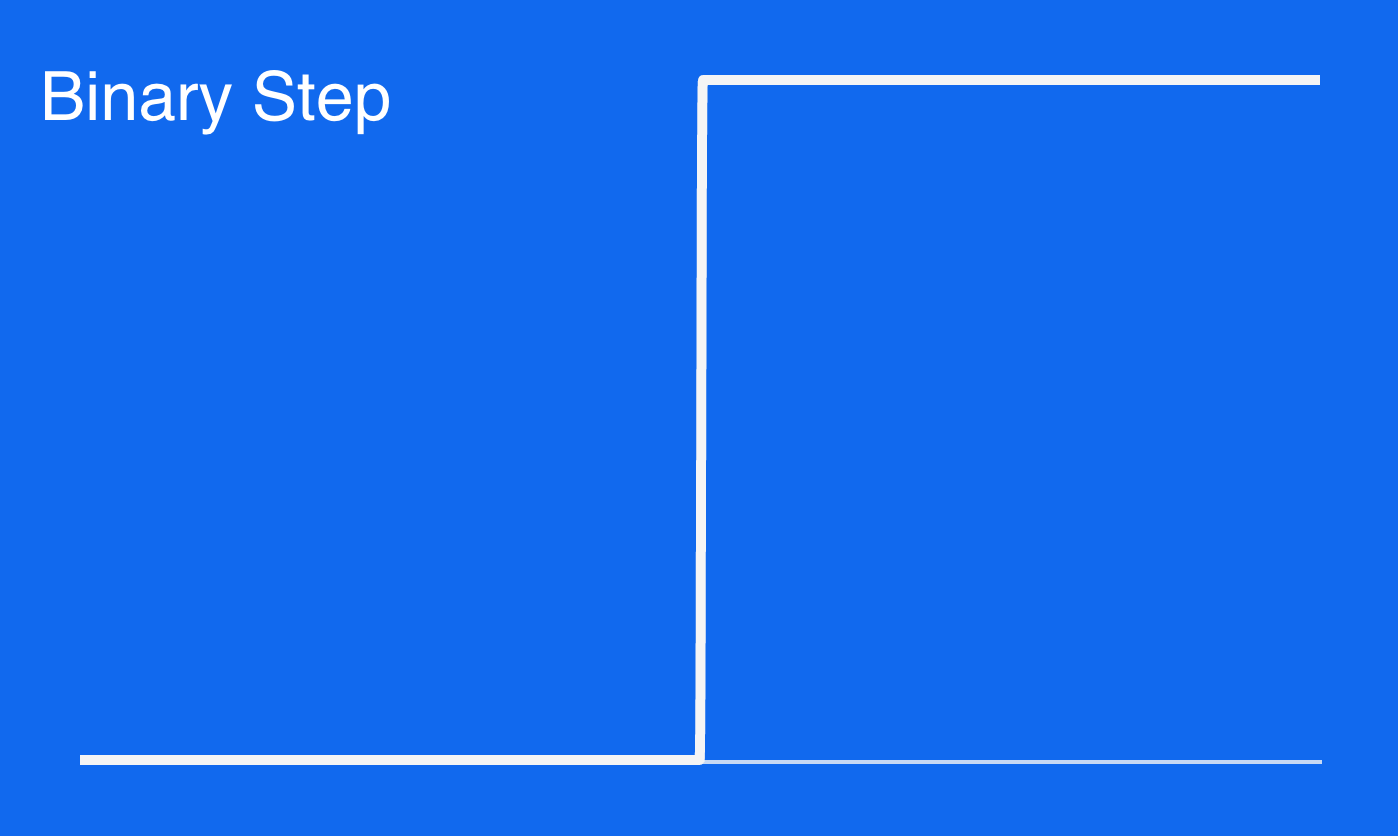
\includegraphics[width=.265\textwidth]{4fig/binary.png}
\caption{Binary Step activation function.}
\end{figure}



\section{Linear}.\\\\

This produces a signal proportional to the input multiplied by each neurons weight. It is an improvement over the step function as it allows for multiple outputs. It does however mean that we are unable to use backpropagation (gradient descent) to train the model. In adition to not being able to improve a model, all the layers in the neural network collapse into a single layer. This means that the final layer will always be a linear function of the first layer. This eliminates all the merits which may be gained from deep learning. A neural network with a linear activation function is simply a linear regression model.

\begin{equation}
    f(x) = m(x)
\end{equation}
\begin{figure}[H]
\centering
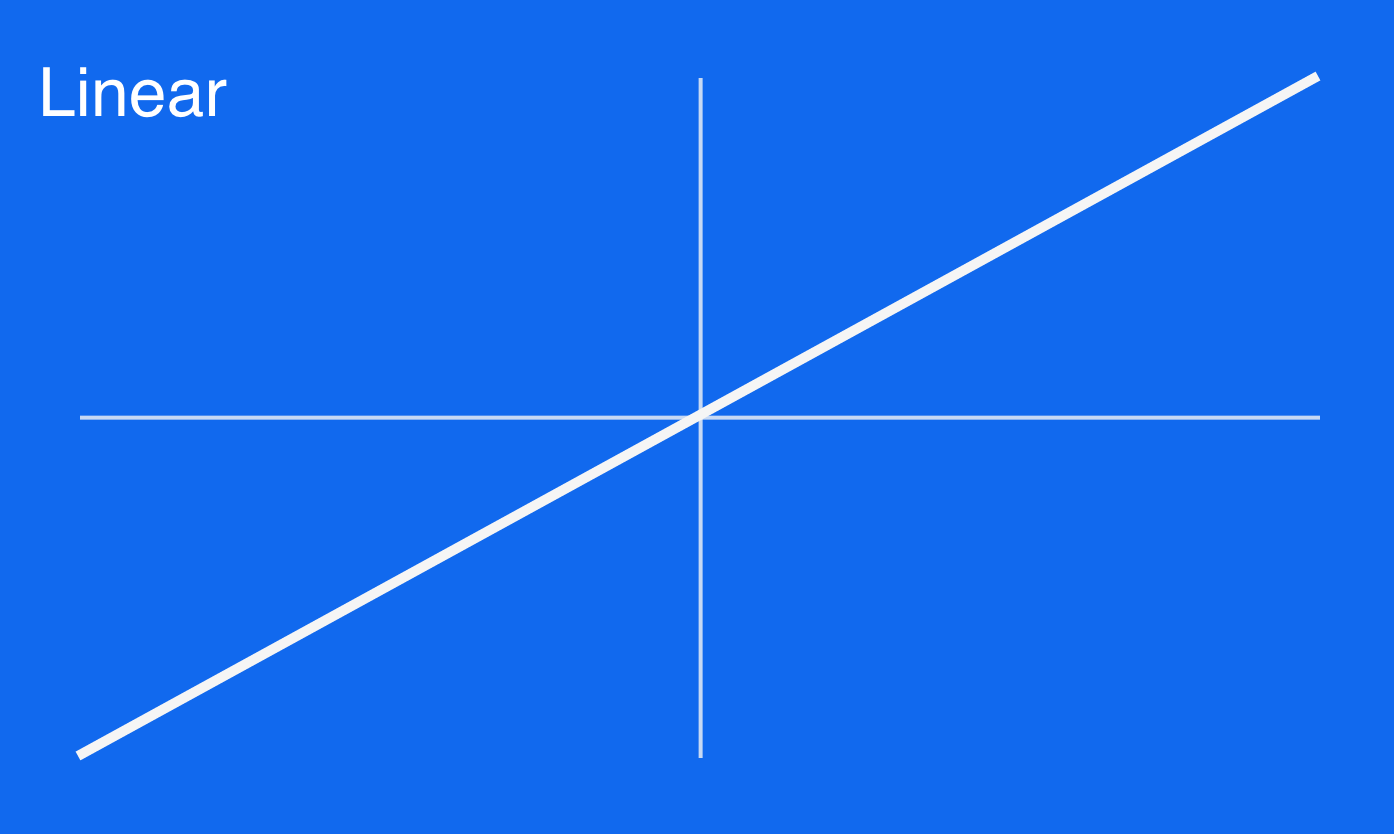
\includegraphics[width=.265\textwidth]{4fig/linear.png}
\caption{Linear activation function.}
\end{figure}

\section{Sigmoid / Logistic}.\\\\
The first of the non-linear activation functions. It has a smooth gradient providing smooth output values which are bound between 1 and 0, normalising the output of each neuron. The main disadvantage is that is falls foul the vanishing gradient problem - for extreme values of $x$ there is close to no change in the prediction. This may result in either early termination of the training, or a slow training cycle in obtaining adequate precision. The activations is computationally expensive and the outputs are not zero centred.

\begin{equation}
    f(x) = 1/1+e^x
\end{equation}
\begin{figure}[H]
\centering
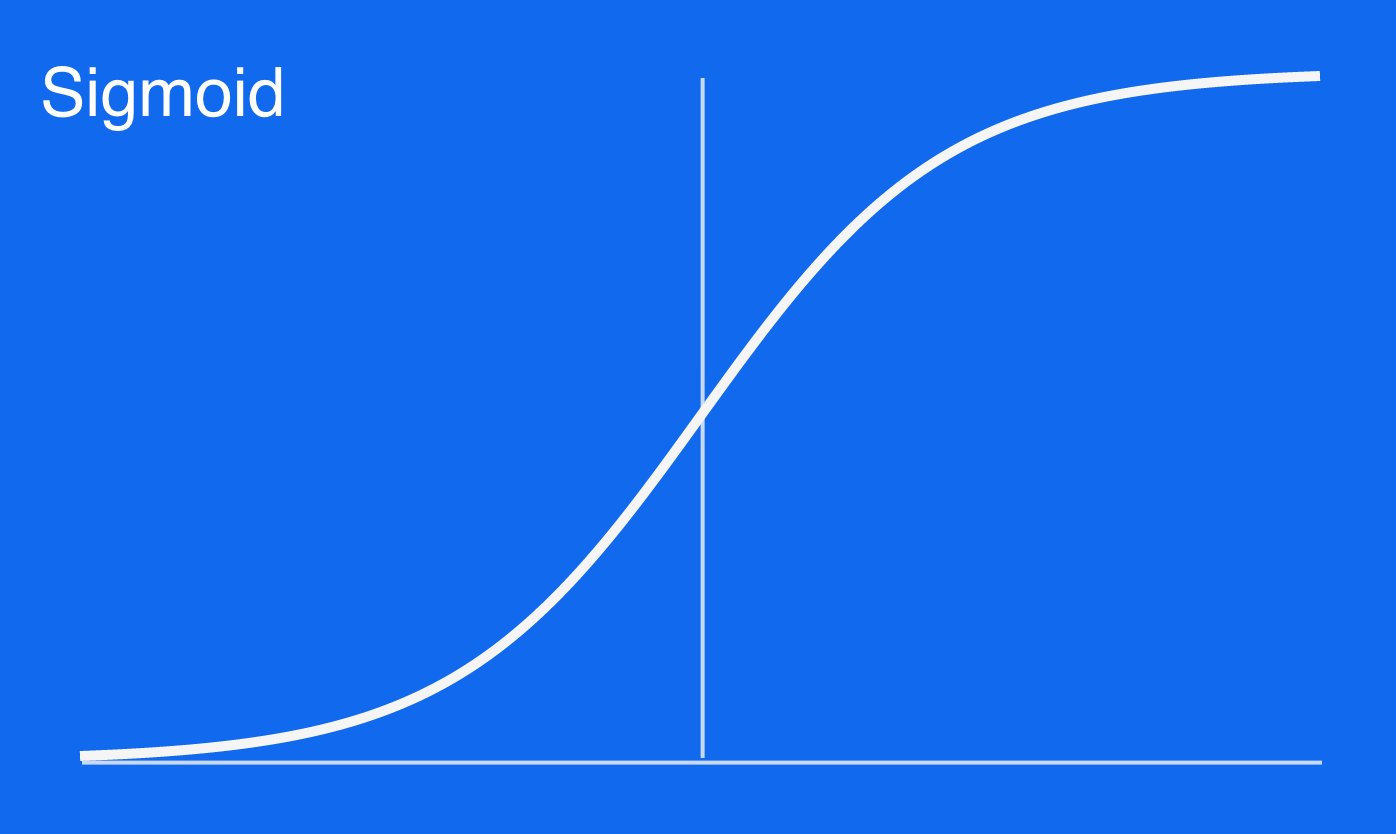
\includegraphics[width=.265\textwidth]{4fig/sigmoid.png}
\caption{Sigmoid activation function.}
\end{figure}


\section{Hyperbolic Tangent}.\\\\
Much like the sigmoid function in both advantages and disadvantages. The hyperbolic tangent function provides a smooth curve which is zero centred. It is however computationally expensive and suffers from the vanishing gradient problem.

\begin{equation}
    f(x) = \frac {e^x - e^{-x}} {e^x + e^{-x}}
\end{equation}
\begin{figure}[H]
\centering
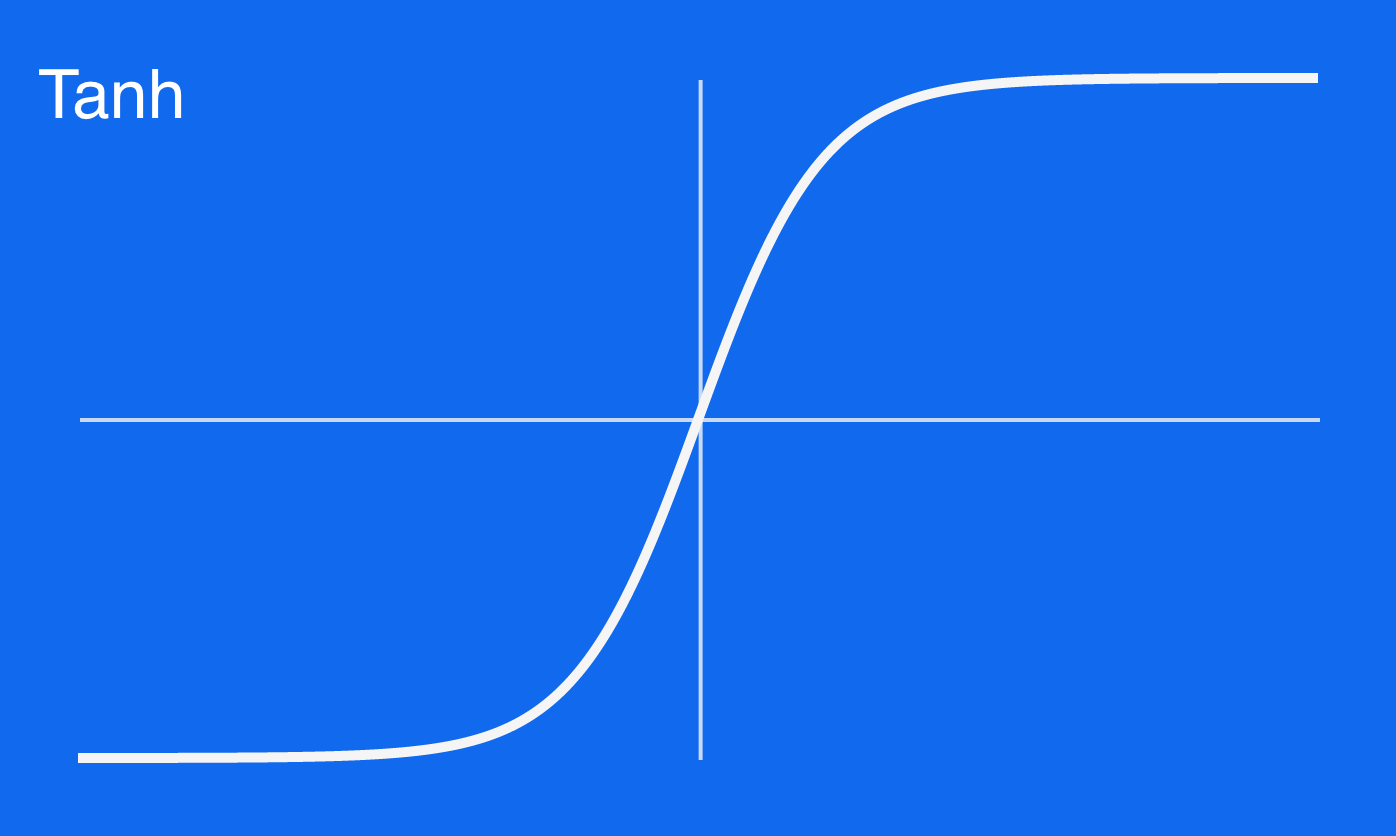
\includegraphics[width=.265\textwidth]{4fig/tanh.png}
\caption{Tanh activation function.}
\end{figure}


\section{Rectified Linear Unit}.\\\\
A commonly used activation for large deep neural networks, due to its computational efficiency and quick convergence. It is non-linear although it appears like a linear function, and allows for back propagation. It does however suffer from the dying ReLU problem - when inputs tend to zero or below, the gradient of the function becomes zero and the network cannot perform backpropagation to learn.

\begin{equation}
f(x) =
    \begin{cases}
      0 , & \mathbf{if} \ x < threshold \\
      x , & \text{otherwise}\\
    \end{cases}
  \end{equation}
\begin{figure}[H]
\centering
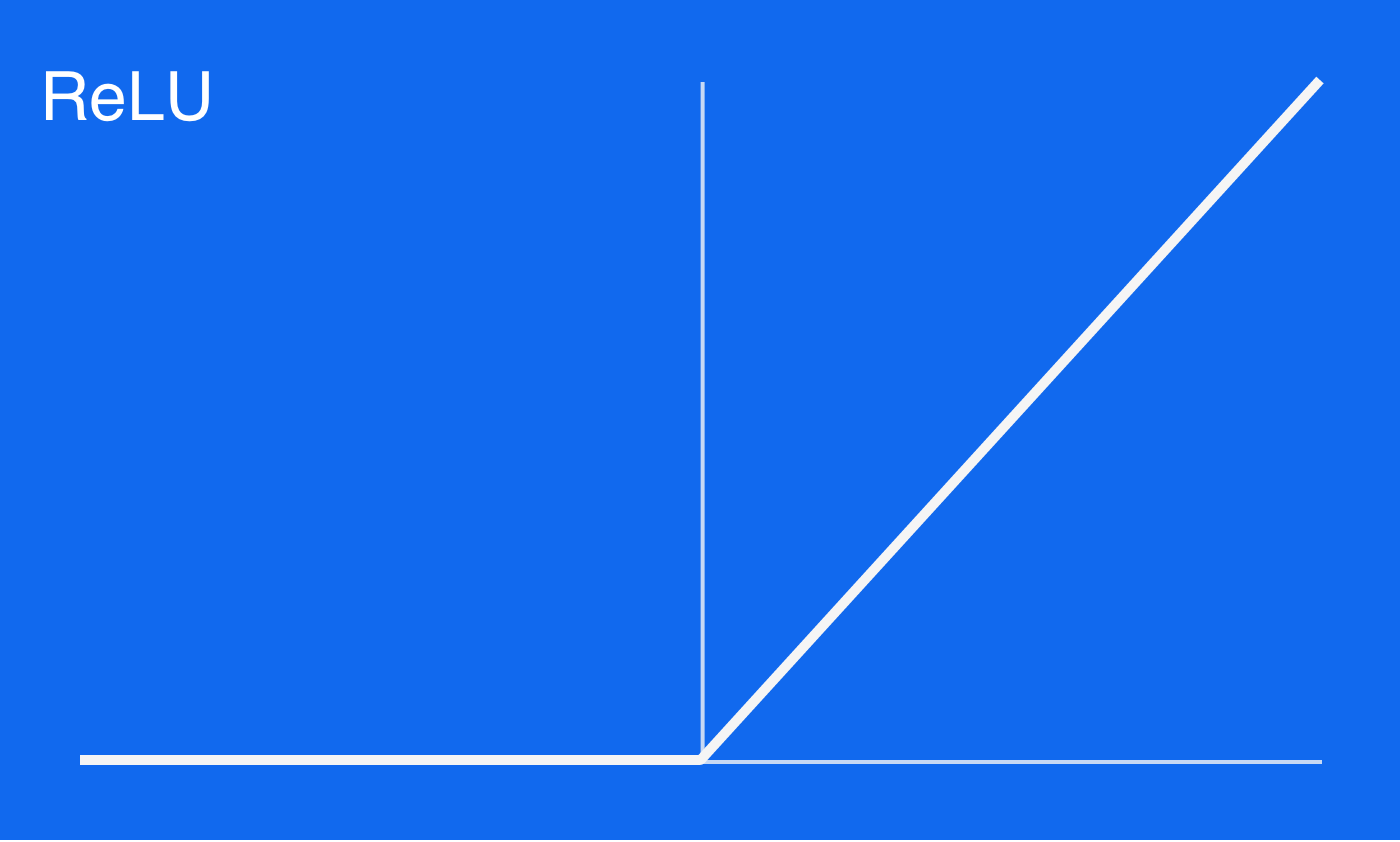
\includegraphics[width=.265\textwidth]{4fig/relu.png}
\caption{ReLU activation function.}
\end{figure}



\section{Swish}.\\\\
https://arxiv.org/abs/1710.05941v1
\textbf{\textit{a new, self-gated activation function discovered by researchers at Google. According to their paper, it performs better than ReLU with a similar level of computational efficiency. In experiments on ImageNet with identical models running ReLU and Swish, the new function achieved top -1 classification accuracy 0.6-0.9\% higher.}}

\begin{equation}
f(x) = x/1-e^{-x}
  \end{equation}
\begin{figure}[H]
\centering
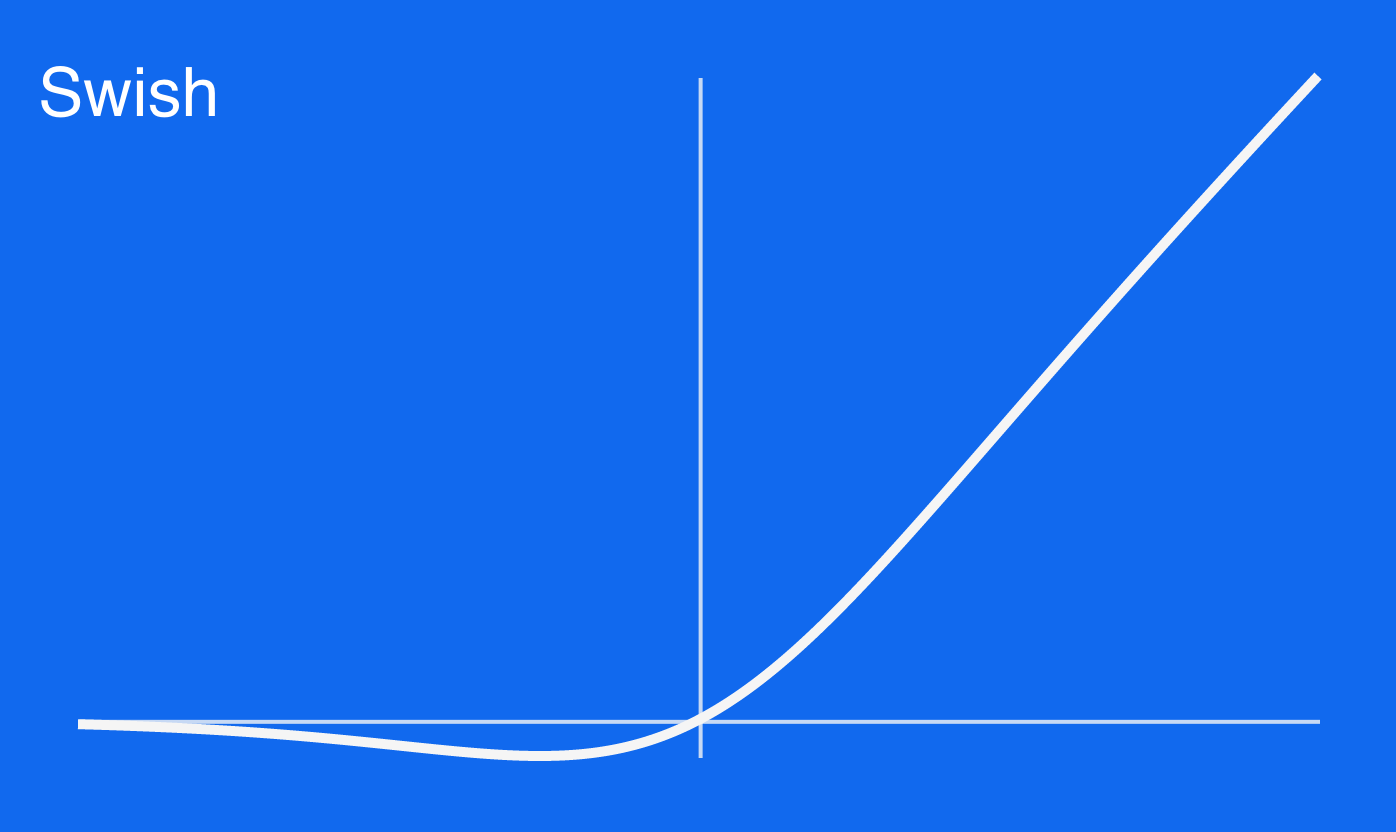
\includegraphics[width=.265\textwidth]{4fig/swish.png}
\caption{Swish activation function.}
\end{figure}

\section{\textbf{A note on backpropagation}}
\emph{As it has not been explicitly explained before back-propagation is an algorithm used to train neural networks. The derivative (or gradient) of an activation function is important in the use of back propagation. Here the model weights are adjusted, and improved, by tracing back all the connections in network, suggesting an optimal weight of each neuron.}
